\documentclass[12pt,english]{article}
\usepackage{mathptmx}

\usepackage{color}
\usepackage[dvipsnames]{xcolor}
\definecolor{darkblue}{RGB}{0.,0.,139.}

\usepackage[top=1in, bottom=1in, left=1in, right=1in]{geometry}

\usepackage{amsmath}
\usepackage{amstext}
\usepackage{amssymb}
\usepackage{setspace}
\usepackage{lipsum}

\usepackage{dcolumn}   % For aligning columns on the decimal point
\usepackage{booktabs}  % For enhanced rules for tables
\usepackage{siunitx}   % For typesetting numbers and units
\usepackage{longtable} % Required for longtable environment


\usepackage[authoryear]{natbib}
\usepackage{url}
\usepackage{booktabs}
\usepackage[flushleft]{threeparttable}
\usepackage{graphicx}
\usepackage[english]{babel}
\usepackage{pdflscape}
\usepackage[unicode=true,pdfusetitle,
 bookmarks=true,bookmarksnumbered=false,bookmarksopen=false,
 breaklinks=true,pdfborder={0 0 0},backref=false,
 colorlinks,citecolor=black,filecolor=black,
 linkcolor=black,urlcolor=black]
 {hyperref}
\usepackage[all]{hypcap} % Links point to top of image, builds on hyperref
\usepackage{breakurl}    % Allows urls to wrap, including hyperref

\linespread{2}

\begin{document}

\begin{singlespace}
\title{Global Warming and Tornado Alley
\thanks{Acknowledgements here, if any.}}
\end{singlespace}

\author{Adam Spohn\thanks{Department of Economics, University of Oklahoma.\
E-mail~address:~\href{mailto:spohn@ou.edu}{spohn@ou.edu}}}

% \date{\today}
\date{\today}

\maketitle

\begin{abstract}
\begin{singlespace}
This paper investigates the possible spatial changes of Tornadoes, and how they may be related to a warming climate. This investigation is done using econometrics methods, including using linear regressions. Findings from this paper can insinuate what possible weather consequences can appear as a result of human behavior, and changes that may need to be made in investment of infrastructure in areas that could be newly impacted by tornadoes.
\end{singlespace}

\end{abstract}
\vfill{}


\pagebreak{}


\section{Introduction}\label{sec:intro}
\hspace{1cm} This paper seeks to find the existence of a shift in tornado occurrences, and if one exists try to investigate a possible relationship between this shift and warming temperatures. This topic is of personal interest to me as someone who is from around the traditional "tornado alley". I have also frequently heard that it was shifting so I wanted to investigate if this was true. Much more recently I had heard arguments that this is a result of global warming, so I thought this could be an interesting relationship to pursue. I believe that these are both important questions to answer. If there is a new geographic area and new populous that is starting to receive more tornadoes, or will receive more tornadoes in the future, they may not be as prepared as a tornado alley populous that has been seeking shelter from them for so long. It would also be important to know whether they had an odd year or two where they received more, or if they should be expecting to continuously be receiving more in the future. Additionally, if a trend like this does in fact exist, understanding whether it is just the result of a natural cycle, or the result of human activity or climate change is important as well. If it is a result of climate change, that might mean that there are changes we could make in our behavior that could lend to differences in tornado behavior. It would be bold to assume that we could start controlling them just by changing our behavior, but it is still important to try to understand what consequences of it may or may not exist. My paper attempts to answer this question using econometrics, and tests for relationships between historical tornado occurrences, and historical data on weather variables within the United States. 

\section{Literature Review}\label{sec:litreview}

\hspace{1cm} Literature of other research on this topic seems to generally be consistent on this topic. There are many significant findings on changes in frequency of tornadoes. One paper studied shifts in location of tornadoes based on different weather variables, including comparing unusually hot and unusually cold years, using a wide variety of methods, though often making use of composite analysis. One of my own questions is if there is any global warming to have an effect on tornadoes in the first place. That may be complex to exactly answer but the research by Cao, Cai and Zhang does find that there have been an increase in air temperatures in the United States over the last few decades, and these differences in air temperatures are what they used to test the effect of warming temperatures on tornado locations. finds that "over the latest 30-year warming period stronger tornado activities have made a statistically-significant geographic shift eastward, northeastward, and southeastward."\cite{Cao2021} On top of shifting tornado activity, it also discusses how supporting elements to make a tornado such as low warm centers and low pressure zones are also shifting. Lastly, this paper mentions that there is a relationship between a warming climate and tornado activity, but it is difficult to determine whether this is a result of natural cycles, or human influence, a question that would be important to answer to decide if there are possible responses to this research. \\
Another paper used observations of tornado locations and tornado supporting environments in a Thiel-Sen Slope analysis in order to observe any shifts over time. They used something called STP (Significant Tornado Parameter) as an indicator of tornado environments. STP is an index of conditions that can lead to F2-F5 scale tornadoes\cite{noaa}. The Thiel-Sen analysis found that "Both tornado reports and environments indicate significant decreasing trends in frequency over portions of Texas, Oklahoma, and northeast Colorado[and]...significant increasing trends in portions of Mississippi, Alabama, Arkansas, Missouri, Illinois, Indiana, Tennessee, and Kentucky."\cite{Vittorio2018}  This research was mainly focused on the shift in tornado occurrences, and did not have findings in relation to being caused by climate change, but it does compliment the previous paper that tornado observations do seem to be shifting. Furthermore both papers appear to be in agreement that it is an eastward shift, along with southeastward and northeastward movement as well. Confirming that this shift is in fact happening was another significant finding for my own research. Though this research pointed out that the southeast may be a vulnerable population to tornadoes, thus important to respond in some way to this new increase. \\
Now that we have shown with confidence that a shift in locations is happening, I want to discuss a paper by Nouri, Devenini, Were and Khanbilvardi that tries to explain these trends. One of their focuses was on the difficulty in older decades to collect tornado data, so they use Doppler radar installations as measure of better detection, and population density is also used as a human factor that may have effected observations. Another notable group of variables this paper used is a lot of environmental variables such as an El-Nino Oscillation variable. I do not have such variables in my own research. Their research used a hierarchical Bayesian inference framework, and they found that "The two anthropogenic covariates explained 17\%, 28\%, and 19\% of the variance in the annual tornado frequency on average across Tornado Alley, Dixie Alley, and Other States,[and]...climate covariates brought additional explanation in the order of 15\%, 11\%, and 5\% on average in the three groups, respectively raising their total average explained variance to 32\%, 40\%, and 24\%."\cite{Nouri2021} They summarized that Population Density was a significant predictor for "Dixie Alley" states but not "tornado alley" states. In turn Doppler Radar installations were the best explanation for trends in tornado alley. This seems to infer that modern differences has had a pretty significant impact on observational trends. Though with that being said there does still seem to be a large impact played by the climate as well.This paper does not explicitly focus on changing temperatures as a large factor of changing trends, but temperature is a part of a complex system that is our climate. As an Oklahoman, another notable comment to me on this paper was that Oklahoma was one of the highest states in variability in tornadoes per year.\\ 
There do appear to be other differences in recent tornado appearances. A study by Moore and DeBoer focuses on differences in the rate at which tornadoes are occurring on a given day, along side the spatial shift. While they are not certain why, they found that "the number of days per year with at least one (E)F1+ tornado decreased between 1954 and 2013 whereas the number of days per year with more than 30 increased."\cite{Moore2019} One interesting thing about this is how it relates to the spatial shift we have seen pointed out in all the other literature. These increases in big tornado days seem to be focused in the southeast, and appears to play a large part in explaining the greater amount of tornado appearances over the amount seen in the Great Plains. "The annual count of (E)F1+ tornadoes in the SE \& [lower Midwest] significantly increased when all (E)F1+ tornadoes are considered...when those that occurred on the big days are removed, however, the increasing trend goes away."\cite{Moore2019} One theory discussed by this paper was that Arctic warming is causing an increase in tornado activity due to a connection between arctic conditions and mid-latitude severe weather reactions. This is something I had heard about before and led me to this research topic. It is only theorized and not proven, though it would have great significance in relation to global warming if it were true. As far as my own testing goes I do not have arctic data, so I will not be able to observe this. Lastly, one thing they did with their data was exclude EF(0), because they especially reflected increasing trends as a result of better detection methods, so I thought this would be important to consider in my own research. 
    

\section{Data}\label{sec:data}
The primary source of tornado data for this research comes from a data table from Kaggle\cite{Bryant2023}, whose data was collected from the NOAA's Storm Prediction Center. Some important variables that come from this data set are the year it came from, the fips code that allows us to track the data at the county level, the F or EF scale, and coordinates that allow for precise mapping and location information. Additionally, I have a data set from GitHub\cite{github} on historical county level temperatures and precipitation. Variables from this data set includes monthly averages for daily highs and daily lows in temperature in degrees Celsius for the months of January and July. The other significant variable from this data set is the average daily amount of precipitation in January or July in millimeters. The summary statistics are for the merge of these two data sets are in Table 1.
This data has the same issue as mentioned in many of the other papers in the literature review, that technology for making tornado observations has improved, which would bias the number, and potentially location of observations over time. I hope to mitigate this issue by removing the observations where there is a 0 for the EF scale. This is because, as suggested by the literature review, these observations may skew the data the most in relation to technology improvements. An alternative method would be to only use more recent years, and I tried this alongside excluding EF0's and tried comparing them later.Summary statistics for these two sub data sets are in table 2 and table 3. A separate issue with the data is that it uses the F (Fujita) scale up to a certain date, then it uses the EF (Enhanced Fujita) scale from that date forward. However, I do not use or compare the EF scales much in my analysis outside of excluding the EF0s, so this should not necessarily be an issue for this project.\\
In order to try to look at whether this data displays any spatial shifts in tornado occurrences, I plotted their mean longitude and latitude over time in graph 1 and graph 2. 



\section{Empirical Methods}\label{sec:methods}
The main model I used in this project is represented in the following equation:

\begin{equation}
Y_{it} = \alpha_0 + \alpha_1 Z_{it} + \alpha_2 W_{it} + \alpha_3 X_{it} + \varepsilon_{it}
\end{equation}
\hspace{1cm} Where $Y_{it}$ represents the longitude or latitude coordinate of a tornado event $i$ in year $t$, $Z_{it}$ represents the mean maximum temperature in July for the tornado event $i$ in year $t$, $W_{it}$ represents the mean precipitation in July for the tornado event $i$ in year $t$, and $X_{it}$ represents the year in which the tornado event $i$ occurred. The parameters of interest are $\alpha_1$, $\alpha_2$, and $\alpha_3$, which capture the effects of mean maximum temperature in July, mean precipitation in July, and year, respectively, on the tornado longitude or latitude coordinates for a specific event in a specific year.\\
I ran this model with three different data sets. My entire data set, a subset of that data set excluding EF0s, and a subset of that data set excluding pre-1970. 


\section{Research Findings}\label{sec:results}
The results from my whole data set are reported in Table 4.
The estimate alpha one can be interpreted as an increase in one degree Celsius of the mean of the daily max temperatures in July would be met with a westward shift in the longitude by 0.306 degrees and a southward shift in latitude by 1.399 degrees of a tornado's occurrence.\\
The estimate alpha two can be interpreted as an increase in one unit (need to find out meaning of unit) of precipitation in July would be met with a eastward shift of 1.960 degrees and a southward shift of 0.966 degrees of a tornado's occurrence.\\
The estimate alpha 3 can be estimated as the change in longitude or latitude in exact units that occurs as a result of a tornado occurring in that year. Notably positive numbers reflect east or north, and negative units reflect west or south. As an example, the 1951 factor variable shows a 0.330 degree shift east, and 2.460 degree shift north. Observing this estimate over each year should give us a picture of how tornado occurrences are shifting over time, excluding climate effects. I believe this should represent what was called in the literature review a natural cycle. Of course, there are many factors not being considered that could effect this, so it may be better to call it a naive natural cycle\\
Based on the results of these estimates, we seem to observe possibly significant effects. alpha 1 was found to be significant at the 99.9\% level, and suggests a southwestward movement, with more southward movement than westward. This was a surprising effect, because I did not expect to find effects that would be shifting westward, though it is not the only effects at play. The precipitation variables were also found to be significant at the 99.9\% level. It had the opposite longitudinal effect than temperature, but a complimentary latitudinal effect. I do not personally have enough meteorological knowledge to know whether this would make sense or be a cause of concern. Each of the factor variables had varying degrees of significance, though they are frequently significant. They vary in estimation as well though the vast majority of them show a eastern shift and a northern shift, only two years showed significant movement westward, and only one year showed significant movement southward. The eastern shift particularly I think should be expected, especially if the climate variables are not necessarily suggesting eastward movement, because the literature review heavily suggested significant eastward movement, so it would be unusual if we did not find any evidence of it here. If there is in fact eastward movement than this model seems to suggest that it is mostly a natural cycle of time as opposed to being caused by global warming. Perhaps alongside this, precipitation is a much more significant factor in eastern movement as opposed to temperature, which also does not support a theory that global warming is causing this eastern shift that has been observed. Again, that is not to say temperature has no effect, though solely based off this model it appears that it has the opposite effect that I was expecting and it is other factors that is making the generally observed change. In turn, the latitudinal results are interesting as well. The literature review seemed to tell us that observations should be moving in both directions, though the year variables seemed to suggest only northward movement. This could mean that the increase in the lower Midwest is a result of a natural cycle, and the result in the southwest is represented by changes in climate, or this model could be doing poorly at representing this change. Regardless, the year variables do show opposite effects than both climate variables for latitude in this model.\\
There are however, potential issues with this model. For one, the R squared for longitude is quite low, so it may be hard to trust the results, or we may want to look for a way to improve it. Also, weather is a very complex system, so the climate variables I used may not reflect the whole picture on their own. Additionally, it may be that it is more of a global system, which would not get represented only looking at United States climate data. For example, the arctic warming that was discussed earlier, or if some other similar relationship could be happening as a result of climate in Mexico or even Europe. Furthermore, there are some variables that represent large weather systems (such as El Nino Southern Oscillation) that is found in some of the literature review, but I do not have data for, nor do I really understand. These are specific examples of additional climate variables that may have an impact when excluded. The hope is that even if it is not a direct representation, that looking at United States climate differences would still reflect some of these differences. Another issues that has been mentioned previously is the differences in observations in older data than more modern data, which is likely caused by improved technology such as Doppler radar, and increased population density. One potential solution I had was to remove EF0 scale tornadoes, under the idea that these may be the hardest to pick up and thus the most effected by new technology. I ran the above model using this new data set. To take a step further I also excluded data prior to 1970 and ran the same model using that data set. Results for the 1970 on and EF(1) plus data are in table 5. Looking at the results there temperature and precipitation have the same direction of predictions, and stayed highly significant, but the year factor variables were flipped in some cases. I am unsure why the year variable so consistently flipped for longitude, but I thought this could be an example of Simpson's paradox. Latitude on the other hand was half in half on flipping in direction or not from the other model. The R squared as well changed. The longitude R squared actually got worse in the new model, though the latitude R squared was better in the new data set's model which excluded EF0s and old data. In relation to the Simpson's paradox, I am not sure which direction should be trusted, but I thought it was even more unusual that the new model would find both that increased temperatures has a westward effect, and that most all years have a westward effect as well, because all other studies suggest eastward movement, and very little of that is being shown in the new model. Regardless, I decided to plot the year's estimates, added to the intercept, alongside some other steps to shift it towards the mean, in order to plot the naive natural cycle suggested by this model. This plot can be found in Graph 3.

\section{Conclusion}\label{sec:conclusion}
\hspace{1cm} This paper attempted to find the effect of climate change on spatial shifts in tornado occurrences by linear regression. This regression consists of temperature, precipitation and year as a factor variable regressed over longitudinal latitudinal coordinates. Literature review on this topic suggests an eastward shift, alongside both northward and southward, or just pure eastward shift. There has been much research and less concrete answers on exactly why this is. The difficulty to answer this comes partly from the complexity and lack of total understanding of weather, and partly from the change in ability to observe tornado occurrences over the decades. Many studies suggest the but do not confirm climate effects. My own empirical research found significant, but mixed evidence of an eastward shift as well, coming from precipitation and changes over time. However,increased temperatures represented westward change. Most variables were significant, but the trustworthiness of the model itself may be in question. A likely culprit of this I believe is that the variables used and geographic space they are measured in may be too simple and small of an area to represent a complex global system. Nevertheless, I still believe that it does indicate that climate, including temperature, does have an impact on tornado occurrences, even if we are not certain about what this effect may be. This in turn highlights even greater importance of what is going on with climate change. There are many interacting systems on our earth and severe weather is just one example of something that will have unexpected consequences and changes in response to it, but it does seem to be proven that there are in fact real changes as a result of it.  

\newpage


\section{}
\bibliographystyle{plain} 
\bibliography{references.bib}
\newpage

\section{Tables and Figures}
% latex table generated in R 4.2.3 by xtable 1.8-4 package
% Thu May  2 00:58:59 2024
\begin{table}[ht]
\centering
\caption{Summary Statistics} 
\begin{tabular}{rrrrrr}
  \hline
 & n & mean & sd & min & max \\ 
  \hline
year & 65651.00 & 1990.29 & 18.87 & 1950.00 & 2019.00 \\ 
  mag & 65651.00 & 0.75 & 1.13 & -9.00 & 5.00 \\ 
  slon & 65651.00 & -92.67 & 9.36 & -124.47 & 0.00 \\ 
  slat & 65651.00 & 37.11 & 5.28 & 0.00 & 49.33 \\ 
  mean\_tmax\_jan & 65651.00 & 7.16 & 7.98 & -19.23 & 28.35 \\ 
  mean\_tmax\_jul & 65651.00 & 31.64 & 2.93 & 16.59 & 42.57 \\ 
  mean\_tmin\_jan & 65651.00 & -4.84 & 7.41 & -30.91 & 17.66 \\ 
  mean\_tmin\_jul & 65651.00 & 18.81 & 3.36 & 2.72 & 28.45 \\ 
  mean\_prec\_jan & 65651.00 & 2.01 & 1.88 & 0.02 & 23.81 \\ 
  mean\_prec\_jul & 65651.00 & 3.28 & 1.96 & 0.00 & 17.97 \\ 
  decade & 65651.00 & 1985.67 & 18.76 & 1950.00 & 2010.00 \\ 
   \hline
\end{tabular}
\end{table}

% latex table generated in R 4.2.3 by xtable 1.8-4 package
% Thu May  2 00:59:00 2024
\begin{table}[ht]
\centering
\caption{Summary Statistics for EF1plus dataset} 
\begin{tabular}{rrrrrr}
  \hline
 & n & mean & sd & min & max \\ 
  \hline
year & 35012.00 & 1985.40 & 19.67 & 1950.00 & 2019.00 \\ 
  mag & 35012.00 & 1.48 & 0.73 & 1.00 & 5.00 \\ 
  slon & 35012.00 & -91.21 & 9.24 & -124.20 & 0.00 \\ 
  slat & 35012.00 & 36.91 & 5.15 & 0.00 & 49.33 \\ 
  mean\_tmax\_jan & 35012.00 & 7.18 & 7.74 & -19.23 & 27.90 \\ 
  mean\_tmax\_jul & 35012.00 & 31.62 & 2.88 & 18.56 & 42.57 \\ 
  mean\_tmin\_jan & 35012.00 & -4.62 & 7.16 & -30.91 & 17.46 \\ 
  mean\_tmin\_jul & 35012.00 & 18.96 & 3.17 & 3.77 & 27.44 \\ 
  mean\_prec\_jan & 35012.00 & 2.24 & 1.92 & 0.03 & 23.81 \\ 
  mean\_prec\_jul & 35012.00 & 3.38 & 1.91 & 0.01 & 17.97 \\ 
  decade & 35012.00 & 1980.86 & 19.53 & 1950.00 & 2010.00 \\ 
   \hline
\end{tabular}
\end{table}

% latex table generated in R 4.2.3 by xtable 1.8-4 package
% Thu May  2 00:59:00 2024
\begin{table}[ht]
\centering
\caption{Summary Statistics for EF1plus_recent dataset} 
\begin{tabular}{rrrrrr}
  \hline
 & n & mean & sd & min & max \\ 
  \hline
year & 26161.00 & 1993.81 & 15.13 & 1970.00 & 2019.00 \\ 
  mag & 26161.00 & 1.42 & 0.70 & 1.00 & 5.00 \\ 
  slon & 26161.00 & -90.99 & 8.80 & -124.20 & 0.00 \\ 
  slat & 26161.00 & 36.86 & 5.02 & 0.00 & 49.33 \\ 
  mean\_tmax\_jan & 26161.00 & 7.22 & 7.75 & -17.02 & 27.90 \\ 
  mean\_tmax\_jul & 26161.00 & 31.57 & 2.82 & 18.56 & 42.57 \\ 
  mean\_tmin\_jan & 26161.00 & -4.45 & 7.14 & -30.26 & 17.46 \\ 
  mean\_tmin\_jul & 26161.00 & 19.05 & 3.14 & 3.77 & 26.68 \\ 
  mean\_prec\_jan & 26161.00 & 2.39 & 1.98 & 0.03 & 21.81 \\ 
  mean\_prec\_jul & 26161.00 & 3.40 & 1.90 & 0.01 & 17.97 \\ 
  decade & 26161.00 & 1989.38 & 14.68 & 1970.00 & 2010.00 \\ 
   \hline
\end{tabular}
\end{table}
 
\pagebreak
Graph 1
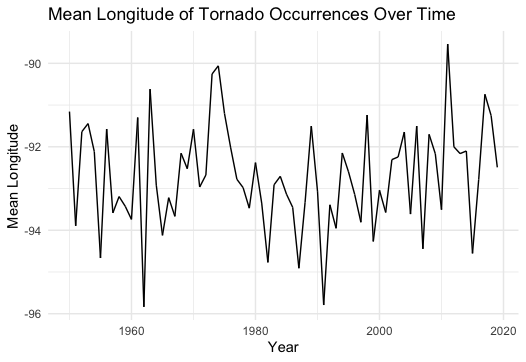
\includegraphics[scale=0.7]{longplot.png}
\newpage
Graph 2
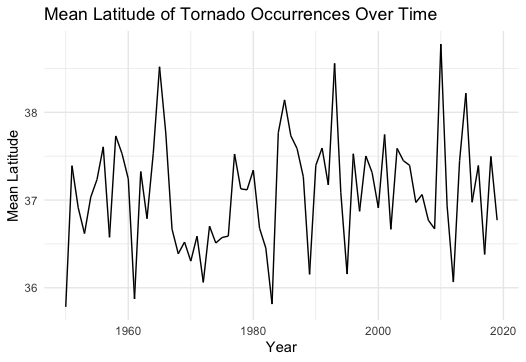
\includegraphics[scale=0.7]{latplot.png}
% Table created by stargazer v.5.2.3 by Marek Hlavac, Social Policy Institute. E-mail: marek.hlavac at gmail.com
% Date and time: Wed, Apr 24, 2024 - 01:34:32
% Requires LaTeX packages: dcolumn 
% Table created by stargazer v.5.2.3 by Marek Hlavac, Social Policy Institute. E-mail: marek.hlavac at gmail.com
% Date and time: Wed, Apr 24, 2024 - 02:55:03
% Requires LaTeX packages: dcolumn 
\renewcommand{\arraystretch}{0.5}
\begin{longtable}[!htbp]{@{\extracolsep{5pt}}lD{.}{.}{-3} D{.}{.}{-3}} 
  \caption{Regression Results} 
  \label{tab:regression_results} \\
  \hline 
  \hline 
  \endfirsthead
  \hline 
  \endhead
 & \multicolumn{2}{c}{\textit{Dependent variable:}} \\ 
\cline{2-3} 
\\[-1.8ex] & \multicolumn{1}{c}{slon} & \multicolumn{1}{c}{slat} \\ 
\\[-1.8ex] & \multicolumn{1}{c}{(1)} & \multicolumn{1}{c}{(2)}\\ 
\hline \\[-1.8ex] 
 mean\_tmax\_jul & -0.308^{***} & -1.399^{***} \\ 
  & (0.012) & (0.005) \\ 
  & & \\ 
 mean\_prec\_jul & 1.960^{***} & -0.966^{***} \\ 
  & (0.018) & (0.007) \\ 
  & & \\ 
 year1951 & 0.330 & 2.460^{***} \\ 
  & (0.783) & (0.320) \\ 
  & & \\ 
 year1952 & 5.451^{***} & 3.545^{***} \\ 
  & (0.798) & (0.326) \\ 
  & & \\ 
 year1953 & 3.470^{***} & 1.707^{***} \\ 
  & (0.712) & (0.291) \\ 
  & & \\ 
 year1954 & 6.305^{***} & 4.737^{***} \\ 
  & (0.689) & (0.281) \\ 
  & & \\ 
 year1955 & 2.654^{***} & 4.059^{***} \\ 
  & (0.682) & (0.278) \\ 
  & & \\ 
 year1956 & 3.999^{***} & 2.356^{***} \\ 
  & (0.694) & (0.284) \\ 
  & & \\ 
 year1957 & 3.387^{***} & 2.803^{***} \\ 
  & (0.654) & (0.267) \\ 
  & & \\ 
 year1958 & -2.085^{***} & 2.226^{***} \\ 
  & (0.683) & (0.279) \\ 
  & & \\ 
 year1959 & 0.033 & 2.004^{***} \\ 
  & (0.678) & (0.277) \\ 
  & & \\ 
 year1960 & 0.187 & 2.190^{***} \\ 
  & (0.677) & (0.276) \\ 
  & & \\ 
 year1961 & 1.752^{***} & 0.914^{***} \\ 
  & (0.665) & (0.272) \\ 
  & & \\ 
 year1962 & -1.226^{*} & 1.695^{***} \\ 
  & (0.672) & (0.274) \\ 
  & & \\ 
 year1963 & 3.892^{***} & 2.325^{***} \\ 
  & (0.704) & (0.288) \\ 
  & & \\ 
 year1964 & 2.893^{***} & 3.829^{***} \\ 
  & (0.667) & (0.272) \\ 
  & & \\ 
 year1965 & 1.189^{*} & 2.102^{***} \\ 
  & (0.650) & (0.266) \\ 
  & & \\ 
 year1966 & 2.690^{***} & 4.021^{***} \\ 
  & (0.682) & (0.279) \\ 
  & & \\ 
 year1967 & 0.983 & -0.032 \\ 
  & (0.648) & (0.265) \\ 
  & & \\ 
 year1968 & 2.149^{***} & 0.536^{*} \\ 
  & (0.672) & (0.274) \\ 
  & & \\ 
 year1969 & 1.228^{*} & 2.814^{***} \\ 
  & (0.678) & (0.277) \\ 
  & & \\ 
 year1970 & 4.661^{***} & 1.166^{***} \\ 
  & (0.672) & (0.275) \\ 
  & & \\ 
 year1971 & 0.593 & 1.271^{***} \\ 
  & (0.650) & (0.266) \\ 
  & & \\ 
 year1972 & 1.352^{**} & 0.234 \\ 
  & (0.662) & (0.271) \\ 
  & & \\ 
 year1973 & 3.282^{***} & 1.857^{***} \\ 
  & (0.638) & (0.261) \\ 
  & & \\ 
 year1974 & 6.518^{***} & 1.552^{***} \\ 
  & (0.647) & (0.264) \\ 
  & & \\ 
 year1975 & 1.801^{***} & 1.710^{***} \\ 
  & (0.648) & (0.265) \\ 
  & & \\ 
 year1976 & 2.712^{***} & 0.657^{**} \\ 
  & (0.654) & (0.267) \\ 
  & & \\ 
 year1977 & 3.050^{***} & 3.296^{***} \\ 
  & (0.654) & (0.267) \\ 
  & & \\ 
 year1978 & 1.732^{***} & 2.687^{***} \\ 
  & (0.658) & (0.269) \\ 
  & & \\ 
 year1979 & 0.033 & 1.600^{***} \\ 
  & (0.652) & (0.267) \\ 
  & & \\ 
 year1980 & 4.567^{***} & 4.193^{***} \\ 
  & (0.654) & (0.267) \\ 
  & & \\ 
 year1981 & 0.625 & 2.490^{***} \\ 
  & (0.659) & (0.269) \\ 
  & & \\ 
 year1982 & 0.383 & 1.915^{***} \\ 
  & (0.642) & (0.262) \\ 
  & & \\ 
 year1983 & 3.850^{***} & 1.608^{***} \\ 
  & (0.649) & (0.265) \\ 
  & & \\ 
 year1984 & 2.296^{***} & 1.666^{***} \\ 
  & (0.649) & (0.265) \\ 
  & & \\ 
 year1985 & 1.503^{**} & 2.312^{***} \\ 
  & (0.668) & (0.273) \\ 
  & & \\ 
 year1986 & 2.002^{***} & 3.068^{***} \\ 
  & (0.661) & (0.270) \\ 
  & & \\ 
 year1987 & 0.431 & 2.050^{***} \\ 
  & (0.672) & (0.275) \\ 
  & & \\ 
 year1988 & 1.724^{***} & 2.551^{***} \\ 
  & (0.667) & (0.273) \\ 
  & & \\ 
 year1989 & 2.153^{***} & 1.089^{***} \\ 
  & (0.652) & (0.267) \\ 
  & & \\ 
 year1990 & 1.394^{**} & 0.916^{***} \\ 
  & (0.637) & (0.260) \\ 
  & & \\ 
 year1991 & -0.683 & 2.063^{***} \\ 
  & (0.638) & (0.261) \\ 
  & & \\ 
 year1992 & -0.996 & 0.147 \\ 
  & (0.630) & (0.258) \\ 
  & & \\ 
 year1993 & -2.021^{***} & 2.377^{***} \\ 
  & (0.635) & (0.259) \\ 
  & & \\ 
 year1994 & 0.917 & 1.097^{***} \\ 
  & (0.639) & (0.261) \\ 
  & & \\ 
 year1995 & 2.253^{***} & 2.028^{***} \\ 
  & (0.633) & (0.259) \\ 
  & & \\ 
 year1996 & 0.620 & 1.274^{***} \\ 
  & (0.636) & (0.260) \\ 
  & & \\ 
 year1997 & 1.228^{*} & 1.120^{***} \\ 
  & (0.637) & (0.260) \\ 
  & & \\ 
 year1998 & 3.554^{***} & 2.342^{***} \\ 
  & (0.628) & (0.256) \\ 
  & & \\ 
 year1999 & 2.039^{***} & 2.278^{***} \\ 
  & (0.631) & (0.258) \\ 
  & & \\ 
 year2000 & 2.665^{***} & 1.525^{***} \\ 
  & (0.641) & (0.262) \\ 
  & & \\ 
 year2001 & 1.479^{**} & 2.999^{***} \\ 
  & (0.634) & (0.259) \\ 
  & & \\ 
 year2002 & 2.439^{***} & 2.306^{***} \\ 
  & (0.647) & (0.264) \\ 
  & & \\ 
 year2003 & 2.478^{***} & 2.387^{***} \\ 
  & (0.628) & (0.257) \\ 
  & & \\ 
 year2004 & 1.704^{***} & 0.418^{*} \\ 
  & (0.618) & (0.253) \\ 
  & & \\ 
 year2005 & 0.684 & 2.682^{***} \\ 
  & (0.632) & (0.258) \\ 
  & & \\ 
 year2006 & 4.126^{***} & 2.937^{***} \\ 
  & (0.639) & (0.261) \\ 
  & & \\ 
 year2007 & 0.269 & 1.172^{***} \\ 
  & (0.639) & (0.261) \\ 
  & & \\ 
 year2008 & 3.270^{***} & 1.854^{***} \\ 
  & (0.621) & (0.254) \\ 
  & & \\ 
 year2009 & 0.813 & 0.305 \\ 
  & (0.635) & (0.260) \\ 
  & & \\ 
 year2010 & 0.140 & 3.343^{***} \\ 
  & (0.631) & (0.258) \\ 
  & & \\ 
 year2011 & 6.233^{***} & 3.833^{***} \\ 
  & (0.621) & (0.254) \\ 
  & & \\ 
 year2012 & 3.916^{***} & 4.112^{***} \\ 
  & (0.648) & (0.265) \\ 
  & & \\ 
 year2013 & 1.305^{**} & 0.855^{***} \\ 
  & (0.648) & (0.265) \\ 
  & & \\ 
 year2014 & 2.966^{***} & -0.924^{***} \\ 
  & (0.651) & (0.266) \\ 
  & & \\ 
 year2015 & 0.047 & 1.972^{***} \\ 
  & (0.635) & (0.259) \\ 
  & & \\ 
 year2016 & 1.330^{**} & 2.937^{***} \\ 
  & (0.645) & (0.263) \\ 
  & & \\ 
 year2017 & 4.118^{***} & 1.569^{***} \\ 
  & (0.627) & (0.256) \\ 
  & & \\ 
 year2018 & 3.637^{***} & 1.628^{***} \\ 
  & (0.637) & (0.260) \\ 
  & & \\ 
 year2019 & 3.026^{***} & 1.596^{***} \\ 
  & (0.625) & (0.255) \\ 
  & & \\ 
 Constant & -91.365^{***} & 82.582^{***} \\ 
  & (0.702) & (0.287) \\ 
  & & \\ 
\hline \\[-1.8ex] 
Observations & \multicolumn{1}{c}{65,651} & \multicolumn{1}{c}{65,651} \\ 
R$^{2}$ & \multicolumn{1}{c}{0.197} & \multicolumn{1}{c}{0.579} \\ 
Adjusted R$^{2}$ & \multicolumn{1}{c}{0.196} & \multicolumn{1}{c}{0.579} \\ 
Residual Std. Error (df = 65579) & \multicolumn{1}{c}{8.390} & \multicolumn{1}{c}{3.428} \\ 
F Statistic (df = 71; 65579) & \multicolumn{1}{c}{226.794$^{***}$} & \multicolumn{1}{c}{1,271.595$^{***}$} \\ 
\hline 
\hline \\[-1.8ex] 
\textit{Note:}  & \multicolumn{2}{r}{$^{*}$p$<$0.1; $^{**}$p$<$0.05; $^{***}$p$<$0.01} \\  
\end{longtable} 
% Table created by stargazer v.5.2.3 by Marek Hlavac, Social Policy Institute. E-mail: marek.hlavac at gmail.com
% Date and time: Thu, May 02, 2024 - 01:45:57
% Requires LaTeX packages: dcolumn 
\begin{longtable}[!htbp]{@{\extracolsep{5pt}}l>{\centering\arraybackslash}D{.}{.}{-3}>{\centering\arraybackslash}D{.}{.}{-3}} 
\caption{Regression Results Sub Data} 
  \label{} 
\begin{tabular}{@{\extracolsep{5pt}}lD{.}{.}{-3} D{.}{.}{-3} } 
\\[-1.8ex]\hline 
\hline \\[-1.8ex] 
 & \multicolumn{2}{c}{\textit{Dependent variable:}} \\ 
\cline{2-3} 
\\[-1.8ex] & \multicolumn{1}{c}{slon} & \multicolumn{1}{c}{slat} \\ 
\\[-1.8ex] & \multicolumn{1}{c}{(1)} & \multicolumn{1}{c}{(2)}\\ 
\hline \\[-1.8ex] 
 mean\_tmax\_jul & -0.458^{***} & -1.413^{***} \\ 
  & (0.019) & (0.008) \\ 
  & & \\ 
 mean\_prec\_jul & 1.604^{***} & -0.923^{***} \\ 
  & (0.028) & (0.011) \\ 
  & & \\ 
 year1971 & -3.883^{***} & 0.148 \\ 
  & (0.471) & (0.186) \\ 
  & & \\ 
 year1972 & -3.179^{***} & -0.988^{***} \\ 
  & (0.493) & (0.195) \\ 
  & & \\ 
 year1973 & -1.831^{***} & 0.846^{***} \\ 
  & (0.451) & (0.178) \\ 
  & & \\ 
 year1974 & 1.537^{***} & 0.474^{***} \\ 
  & (0.466) & (0.184) \\ 
  & & \\ 
 year1975 & -2.812^{***} & 0.816^{***} \\ 
  & (0.487) & (0.192) \\ 
  & & \\ 
 year1976 & -1.984^{***} & -0.245 \\ 
  & (0.487) & (0.192) \\ 
  & & \\ 
 year1977 & -1.750^{***} & 2.383^{***} \\ 
  & (0.483) & (0.191) \\ 
  & & \\ 
 year1978 & -2.603^{***} & 1.677^{***} \\ 
  & (0.520) & (0.205) \\ 
  & & \\ 
 year1979 & -3.920^{***} & 0.367^{*} \\ 
  & (0.510) & (0.201) \\ 
  & & \\ 
 year1980 & 0.179 & 2.783^{***} \\ 
  & (0.488) & (0.192) \\ 
  & & \\ 
 year1981 & -3.374^{***} & 1.366^{***} \\ 
  & (0.509) & (0.201) \\ 
  & & \\ 
 year1982 & -4.051^{***} & 0.722^{***} \\ 
  & (0.474) & (0.187) \\ 
  & & \\ 
 year1983 & 0.041 & 0.360^{*} \\ 
  & (0.490) & (0.193) \\ 
  & & \\ 
 year1984 & -2.318^{***} & 0.508^{***} \\ 
  & (0.499) & (0.197) \\ 
  & & \\ 
 year1985 & -3.037^{***} & 1.014^{***} \\ 
  & (0.546) & (0.215) \\ 
  & & \\ 
 year1986 & -1.915^{***} & 2.294^{***} \\ 
  & (0.533) & (0.210) \\ 
  & & \\ 
 year1987 & -4.824^{***} & 0.880^{***} \\ 
  & (0.576) & (0.227) \\ 
  & & \\ 
 year1988 & -2.333^{***} & 1.497^{***} \\ 
  & (0.533) & (0.210) \\ 
  & & \\ 
 year1989 & -2.191^{***} & -0.273 \\ 
  & (0.511) & (0.202) \\ 
  & & \\ 
 year1990 & -2.448^{***} & -0.246 \\ 
  & (0.486) & (0.192) \\ 
  & & \\ 
 year1991 & -3.668^{***} & 1.227^{***} \\ 
  & (0.523) & (0.206) \\ 
  & & \\ 
 year1992 & -5.202^{***} & -0.830^{***} \\ 
  & (0.490) & (0.193) \\ 
  & & \\ 
 year1993 & -5.614^{***} & 1.761^{***} \\ 
  & (0.527) & (0.208) \\ 
  & & \\ 
 year1994 & -2.306^{***} & 0.036 \\ 
  & (0.544) & (0.215) \\ 
  & & \\ 
 year1995 & -0.520 & 1.009^{***} \\ 
  & (0.532) & (0.210) \\ 
  & & \\ 
 year1996 & -2.396^{***} & 0.109 \\ 
  & (0.530) & (0.209) \\ 
  & & \\ 
 year1997 & -1.579^{***} & -0.104 \\ 
  & (0.537) & (0.212) \\ 
  & & \\ 
 year1998 & 1.188^{**} & 0.809^{***} \\ 
  & (0.498) & (0.196) \\ 
  & & \\ 
 year1999 & -1.677^{***} & 1.079^{***} \\ 
  & (0.504) & (0.199) \\ 
  & & \\ 
 year2000 & -0.933^{*} & 0.027 \\ 
  & (0.559) & (0.220) \\ 
  & & \\ 
 year2001 & -2.280^{***} & 1.319^{***} \\ 
  & (0.535) & (0.211) \\ 
  & & \\ 
 year2002 & -0.190 & 1.326^{***} \\ 
  & (0.576) & (0.227) \\ 
  & & \\ 
 year2003 & -1.664^{***} & 0.901^{***} \\ 
  & (0.510) & (0.201) \\ 
  & & \\ 
 year2004 & -1.862^{***} & -0.648^{***} \\ 
  & (0.488) & (0.192) \\ 
  & & \\ 
 year2005 & -2.931^{***} & 1.532^{***} \\ 
  & (0.523) & (0.206) \\ 
  & & \\ 
 year2006 & 0.057 & 1.861^{***} \\ 
  & (0.530) & (0.209) \\ 
  & & \\ 
 year2007 & -3.741^{***} & 0.313 \\ 
  & (0.531) & (0.209) \\ 
  & & \\ 
 year2008 & -0.945^{**} & 0.819^{***} \\ 
  & (0.468) & (0.185) \\ 
  & & \\ 
 year2009 & -2.837^{***} & -1.001^{***} \\ 
  & (0.521) & (0.205) \\ 
  & & \\ 
 year2010 & -3.058^{***} & 2.267^{***} \\ 
  & (0.503) & (0.199) \\ 
  & & \\ 
 year2011 & 1.533^{***} & 2.708^{***} \\ 
  & (0.448) & (0.177) \\ 
  & & \\ 
 year2012 & 0.063 & 3.395^{***} \\ 
  & (0.553) & (0.218) \\ 
  & & \\ 
 year2013 & -2.862^{***} & -0.568^{***} \\ 
  & (0.535) & (0.211) \\ 
  & & \\ 
 year2014 & -0.863 & -2.630^{***} \\ 
  & (0.535) & (0.211) \\ 
  & & \\ 
 year2015 & -4.155^{***} & 0.826^{***} \\ 
  & (0.511) & (0.201) \\ 
  & & \\ 
 year2016 & -2.284^{***} & 1.566^{***} \\ 
  & (0.533) & (0.210) \\ 
  & & \\ 
 year2017 & -0.075 & 0.300 \\ 
  & (0.464) & (0.183) \\ 
  & & \\ 
 year2018 & -0.302 & 0.539^{***} \\ 
  & (0.510) & (0.201) \\ 
  & & \\ 
 year2019 & -0.964^{**} & 0.248 \\ 
  & (0.472) & (0.186) \\ 
  & & \\ 
 Constant & -80.125^{***} & 83.870^{***} \\ 
  & (0.722) & (0.285) \\ 
  & & \\ 
\hline \\[-1.8ex] 
Observations & \multicolumn{1}{c}{26,161} & \multicolumn{1}{c}{26,161} \\ 
R$^{2}$ & \multicolumn{1}{c}{0.169} & \multicolumn{1}{c}{0.602} \\ 
Adjusted R$^{2}$ & \multicolumn{1}{c}{0.167} & \multicolumn{1}{c}{0.601} \\ 
Residual Std. Error (df = 26109) & \multicolumn{1}{c}{8.035} & \multicolumn{1}{c}{3.170} \\ 
F Statistic (df = 51; 26109) & \multicolumn{1}{c}{103.832$^{***}$} & \multicolumn{1}{c}{772.748$^{***}$} \\ 
\hline 
\hline \\[-1.8ex] 
\textit{Note:}  & \multicolumn{2}{r}{$^{*}$p$<$0.1; $^{**}$p$<$0.05; $^{***}$p$<$0.01} \\ 
\end{tabular} 
\end{longtable} 
graph 3
\includegraphics[scale = 0.8]{predic.plot.png}




\end{document}
